\documentclass[aspectratio=169,usenames,dvipsnames]{beamer}
\usepackage{preamble}
\title{Coding for Humanities, week 1}
\begin{document}

\begin{frame}
 \titlepage
\end{frame}

\begin{frame}{Plan for today}
 \tableofcontents
\end{frame}




\section{Why programming}
\frame{\tableofcontents[currentsection]}
\begin{frame}{Programming: informal understanding}
    \begin{reference}
        Pine (2009). Learn to program. \url{https://pine.fm/LearnToProgram}
    \end{reference}
    \begin{definition}
        ``\structure{Programming} is telling your computer
        how to do something'' (Pine 2009, xii)
    \end{definition}
\end{frame}

\begin{frame}{Why use computers in research?}
	\pause

    \begin{description}
        \item[Automation:] avoid boring work
        \item[Amplification:] analyze more data than humans can handle
        \item[Reproducibility:] share data \& code along with publications
    \end{description}
\end{frame}

\begin{frame}{To program or not to program}
    Computers need to be told what to do:

    \begin{itemize}
        \item Either user tools designed for a particular job
            \begin{itemize}
                \item but: limited to existing functionality
                \item cannot easily repeat a sequence of actions
            \end{itemize}

        \item \dots or create your own programs
            \begin{itemize}
                \item Higher investment to get started
                \item \dots but opens up lots of opportunities
            \end{itemize}
    \end{itemize}
\end{frame}

\begin{frame}{Research workflow}
    \begin{enumerate}
        \item Formulate research question
        \item Collect data
        \item Pre-process data
        \item Analyze data
        \item Draw conclusions
    \end{enumerate}

    \pause
    \dots programming is useful for steps 2--4
\end{frame}

\begin{frame}{Requirements for being a good programmer}
    \begin{itemize}
        \item Anyone can learn how to program
        \item Programming is a challenging activity:
            \begin{itemize}
                \item Analytic thinking
                \item Mental model of computer
                \item Paying attention to detail
            \end{itemize}
        \item Not everyone has the talent to become
            a \structure{good} programmer
    \end{itemize}
\end{frame}

\begin{frame}{Programming workflow in practice}
	\begin{columns}
		\column{0.3\linewidth}
			Many iterations of \dots
			\begin{itemize}
				\item Fail
				\item Fix
			\end{itemize}

		\column{0.7\linewidth}
			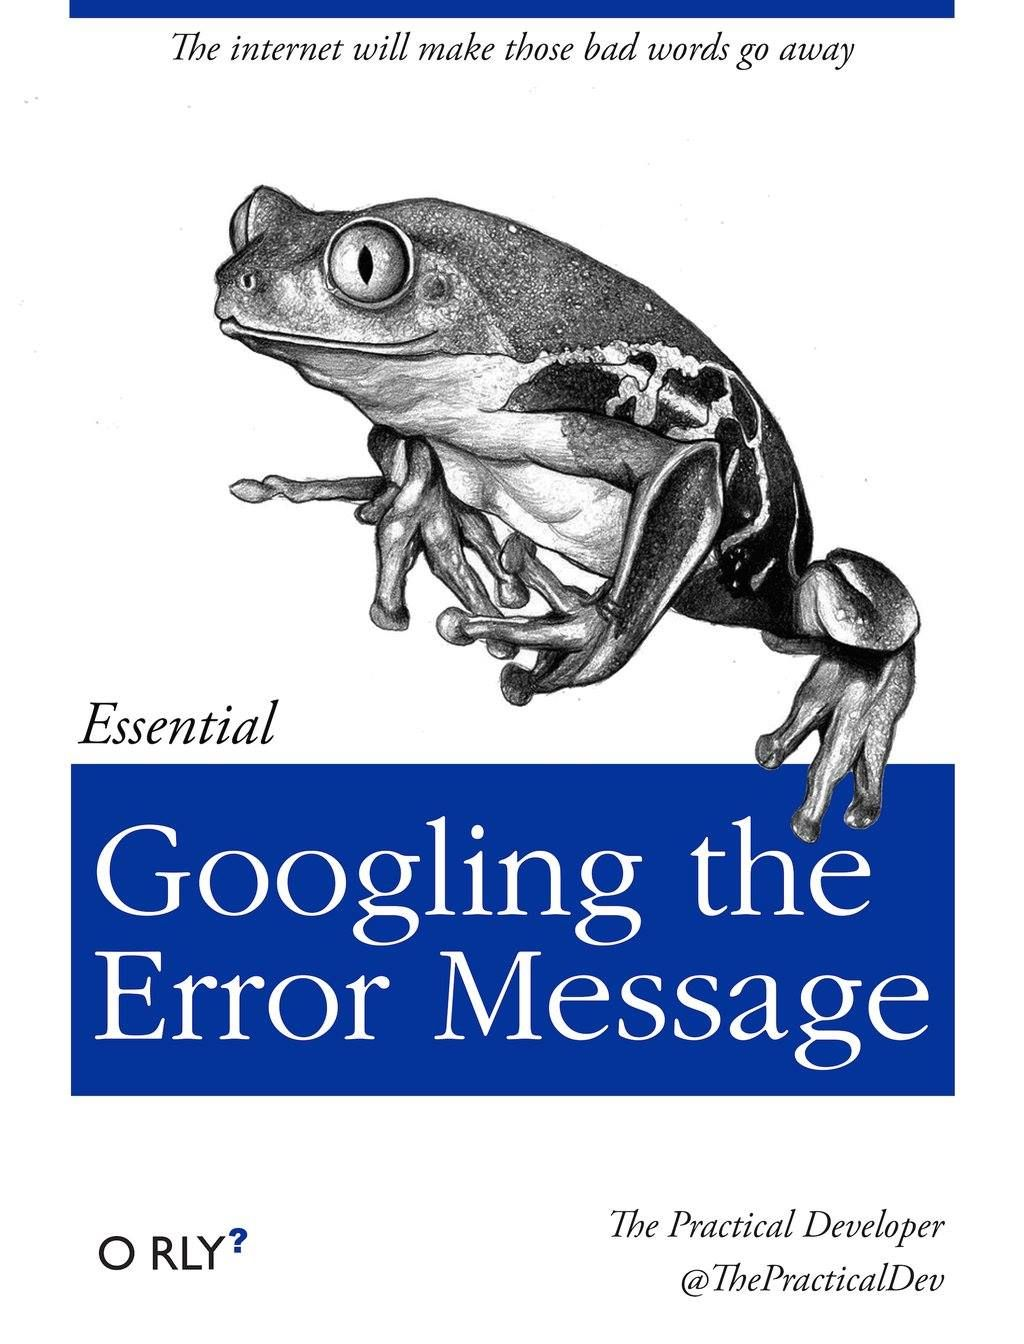
\includegraphics[width=0.45\linewidth]{fig/googling}
			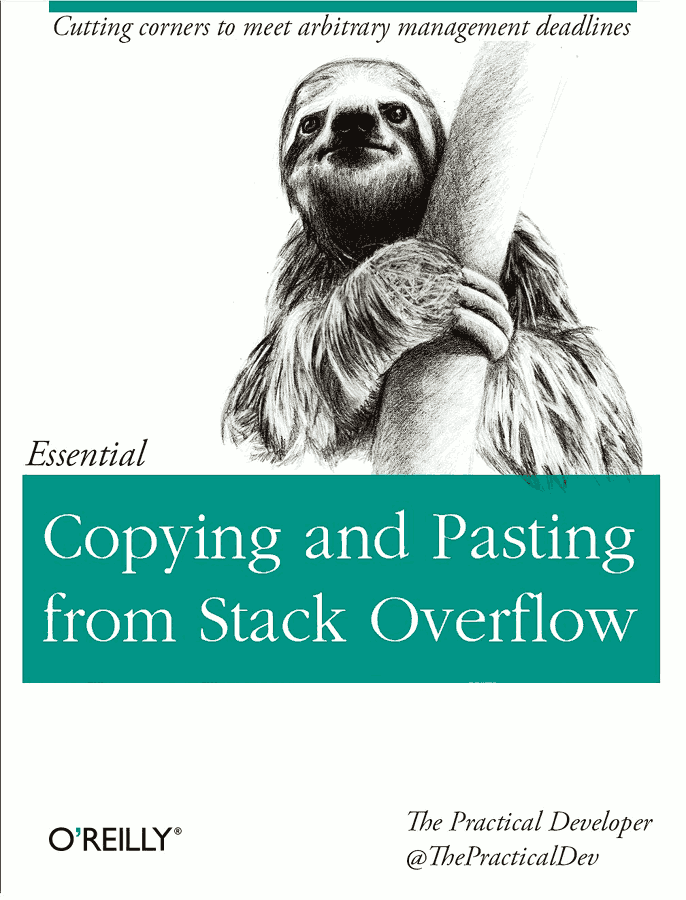
\includegraphics[width=0.45\linewidth]{fig/stackoverflow}
	\end{columns}
\end{frame}



\subsection{Example DH projects}
\frame{\tableofcontents[currentsubsection]}
\begin{frame}{Example DH projects}
\begin{reference}
\url{https://twitter.com/yaelnetzer/status/1158712777776730113}
\end{reference}
    \begin{columns}
        \column{0.5\linewidth}
            Student projects from a DH course by Yael Netzer (Ben Gurion univ.\ Israel):
            \begin{itemize}
                \item Game of Thrones character analysis
                \item Sentiment analysis of GoodReads reviews vs NY times reviews
                \item How many black actors, directors,
                    producers are in movies?
                \item Eurovision song festival voting by country
                %\item Which terror attacks are reported in the NY times?
            \end{itemize}
        \pause
        \column{0.5\linewidth}
            Required skills:
            \begin{description}
                \item[Text analysis] Get texts, extract/filter words, count
                \item[Data science] Get numerical data, explore, plot
            \end{description}
    \end{columns}
\end{frame}

\begin{frame}{Gender in Game of Thrones}\centering
    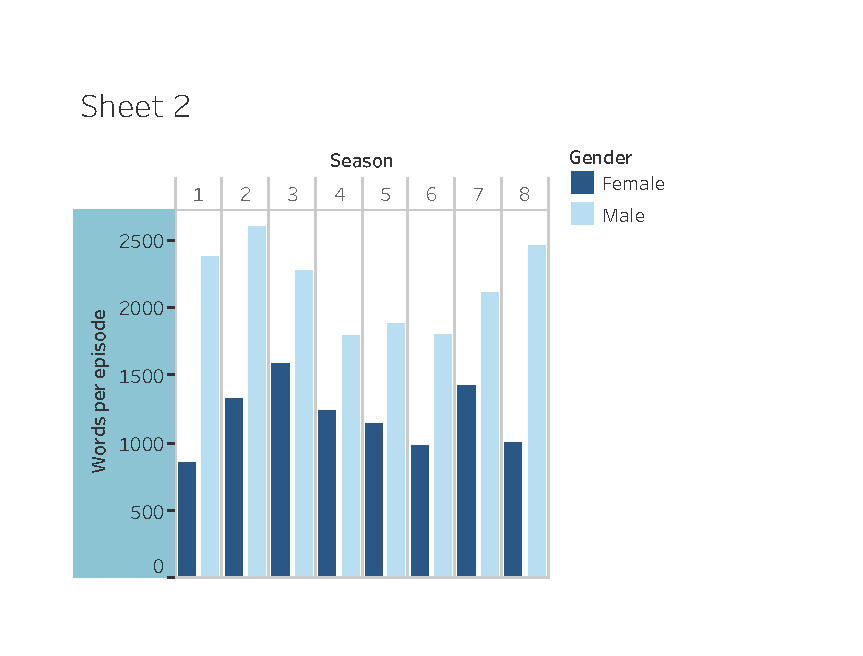
\includegraphics[width=0.6\textwidth]{fig/got}

    Words spoken for each gender across seasons
\end{frame}


\begin{frame}{Intermezzo: female computer pioneers}
	\begin{columns}
		\column{0.3\linewidth}
		Ada Lovelace %, mathematician

		\vspace{1ex}
		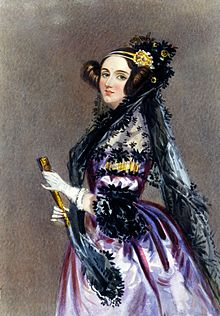
\includegraphics[width=0.9\linewidth,trim={0 1cm 0 1cm},clip]{fig/ada}
		
		Wrote \structure{first computer program}

		\pause
		\column{0.3\linewidth}
		Grace Hopper %, admiral, computer scientist
		
		\vspace{1ex}
		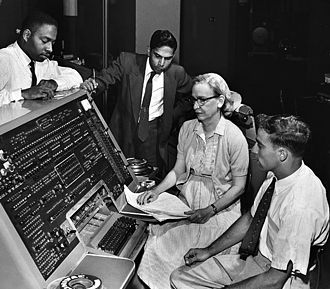
\includegraphics[width=0.9\linewidth]{fig/gracehopper}

		Invented machine-independent \structure{programming languages}

		\pause
		\column{0.3\linewidth}
		Margaret Hamilton %, computer scientist

		\vspace{1ex}
		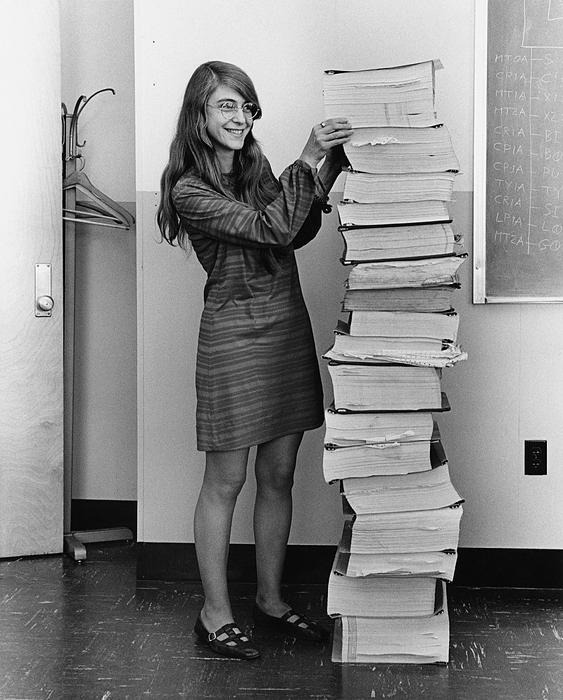
\includegraphics[width=0.9\linewidth]{fig/margarethamilton}

		Lead programmer for \structure{Apollo Moon missions}
		% anecdote of finding bug
	\end{columns}
\end{frame}

\subsection{Why Python}
\frame{\tableofcontents[currentsubsection]}
\begin{frame}{Why Python}
    %\begin{definition}
    %   Python is a  ...
    %\end{definition}
    \begin{itemize}
        \item Easy and intuitive language:
            \begin{itemize}
                \item Code that is understandable as plain English
                \item Ease of development more important than fast programs
            \end{itemize}
        \item Suitable for many tasks:\\
            Many useful libraries (especially data science)
    \end{itemize}

    (Named after the TV show Monty Python)
\end{frame}

\begin{frame}
	% \begin{reference}
	% 	\href{https://www.economist.com/graphic-detail/2018/07/26/python-is-becoming-the-worlds-most-popular-coding-language}{
	% 		The Economist (2018): ``Python is becoming the world's most popular coding language''}
	% \end{reference}

    \centering
    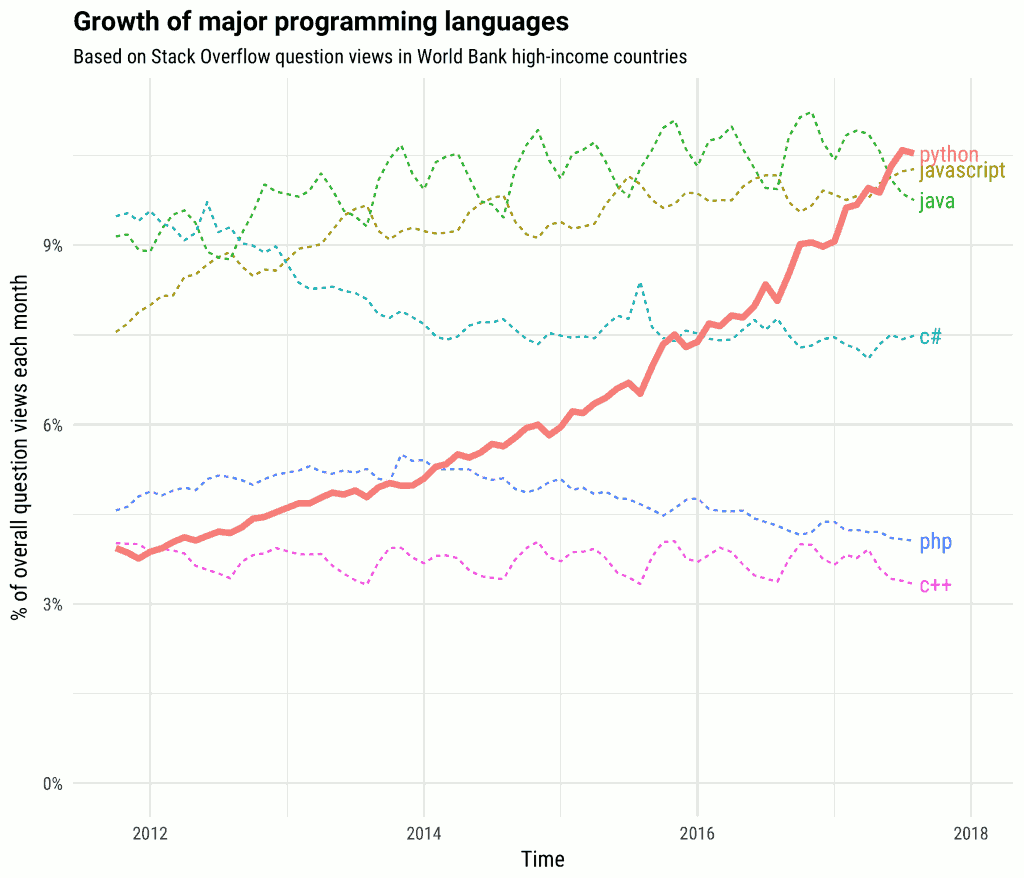
\includegraphics[height=0.9\textheight]{fig/pythongrowth.png}

    Source: \url{https://stackoverflow.blog/2017/09/06/incredible-growth-python/}
\end{frame}

\begin{frame}[fragile]
A simple Python program:
\begin{lstlisting}[language=python]
print('Hello, World!')
\end{lstlisting}

\pause
\vspace{1em}
The same program in the Java programming language:

\begin{lstlisting}[language=java]
public class HelloWorld {
    public static void main(String[] args) {
        System.out.println("Hello, World!");
    }
}
\end{lstlisting}
\end{frame}


\section{Programming fundamentals}
\subsection{Numbers, text, and variables}
\frame{\tableofcontents[currentsubsection]}

\begin{frame}[fragile]{Using Python as a calculator}
Operators:
    \begin{description}
        \item[Addition] 1 + 2
        \item[Subtraction] 2 - 1
        \item[Multiplication] 2 * 3
        \item[Division] 6 / 2
        \item[Exponentation] 3 ** 2
        % \item[Parentheses] (1 + 2) * 3
    \end{description}
\end{frame}

\begin{frame}[fragile]{Using Python as a calculator}
One or more operators can be used to form an \structure{expression}
\begin{lstlisting}[language=python]
In: 1 + 2 * 3
Out: 7
In: (1 + 2) * 3
Out: 9
\end{lstlisting}

\pause
Note:
    \begin{itemize}
        \item As in mathematics, multiplication/division takes precedence over
            addition/subtraction (PEMDAS)
        \item Parentheses can be used to specify a different order.
    \end{itemize}
\end{frame}

\begin{frame}[fragile]{Numeric data types}
    \begin{description}
        \item[Integers] (whole numbers): 1, 2, 3, \dots -1, -2, -3
        \item[Floating point] numbers: 2.5, 1.3333, \dots
    \end{description}

\pause
\begin{lstlisting}[language=python]
In: 5 / 2
Out: 2.5
In: type(5 / 2)
Out: <class 'float'>
In: type(6 / 2)
Out: <class 'int'>
\end{lstlisting}
\end{frame}

\begin{frame}[fragile]{Variables}
    \begin{definition}
        A \structure{variable} stores the result of an expression
        so that it can be re-used.
    \end{definition}

A variable is created/updated using `='

\begin{definition}
\structure{Assignment}: \texttt{name = expression}

\texttt{name} consists of one or more letters or underscores (case-sensitive).
\end{definition}

\begin{lstlisting}[language=python]
In: a = 5 / 2
In: a
Out: 2.5
\end{lstlisting}

(the opposite of a variable is a \structure{constant})
\end{frame}

\begin{frame}{Terminology}
    \begin{description}
        \item[Constant]
            e.g., 2, 5, 1.5, \dots
        \item[Expression]
            A constant, operator, and optionally another expression
            \begin{itemize}
                \item 2 + 5
                \item 1 + 2 + 3
                \item etc.
            \end{itemize}
        \item[Variable] a container that holds a value,
            can be used in place of constants;
            e.g., a, b, books, \dots
    \end{description}
\end{frame}

\begin{frame}[fragile]{Using variables}
Now, can use variable in expressions in place of a number:

\begin{lstlisting}[language=python]
In: a + 0.5
Out: 3.0
\end{lstlisting}

\pause
A program is executed line-by-line, and variables can be overwritten:
\begin{lstlisting}[language=python]
In: a = 2
In: a
Out: 2
In: a = 3
In: a
Out: 3
\end{lstlisting}
\end{frame}

\begin{frame}[fragile]{Updating variables}
A common operation is to increase the value of a variable:
\begin{lstlisting}[language=python]
In: a = 2
In: a = a + 1
Out: 3
\end{lstlisting}

\pause
There is a shorthand for this operation:
\begin{lstlisting}[language=python]
In: a = 2
In: a += 1
Out: 3
\end{lstlisting}

Also -=, *=, etc.
\end{frame}


\begin{frame}{A practical example}
    Suppose I read War \& Peace in a year, \\
    what is my reading speed (words per minute)?
    \begin{itemize}
        \item Number of words in War \& Peace: 564,277
        \item Time spent reading per day: 1 hour
    \end{itemize}
    How to calculate average words per minute?
\end{frame}

\begin{frame}[fragile]{Solution}
\begin{lstlisting}[language=python]
In: words_per_day = 564277 / 365
In: words_per_min = words_per_day / 60
In: words_per_min
Out: 25.766073059360732
\end{lstlisting}
\end{frame}


\begin{frame}[fragile]{Text}
Values can also be text instead of numbers:
\begin{lstlisting}[language=python]
name = 'John'
movie = "2001: A Space Odyssey"
\end{lstlisting}

\pause
    \begin{definition}
        A \structure{string}, short for string of characters,
        is a type of value that contains text.
    \end{definition}
\end{frame}

\begin{frame}{Types}
    We have seen numbers (integer, float) and text (string).

    These are examples of types:

    \begin{definition}
        A \structure{type} is a class of values recognized by the language.
    \end{definition}
    
    \pause
    \begin{itemize}
        \item In Python, a value always has a type (a variable can be any type).
        \item The type determines what operations are valid.
    \end{itemize}
\end{frame}

\begin{frame}[fragile]{Different behavior for types}
    \begin{columns}
        \column{0.5\linewidth}
\begin{lstlisting}[language=python]
In: 3 + 3
Out: 6
\end{lstlisting}

These are \structure{numbers}, so we can do arithmetic
        \column{0.5\linewidth}
\begin{lstlisting}[language=python]
In: '3' + '3'
Out: '33'
\end{lstlisting}

These are \structure{strings}, so they are treated as text
    \end{columns}
\end{frame}

\begin{frame}[fragile]{Invalid operations for types}
\begin{lstlisting}[language=python]
In: 3 + '3'
Traceback (most recent call last):
  File "<stdin>", line 1, in <module>
TypeError: unsupported operand type(s) for +: 'int' and 'str'
\end{lstlisting}
    
    \centering
    
\includegraphics[height=0.5\textheight]{fig/cantdothat}
\end{frame}
    

\begin{frame}[fragile]{Converting numbers to text and back}
\begin{lstlisting}[language=python]
In: number = 42
In: text = str(number)
In: text
Out: '42'

In: int(text)
Out: 42
\end{lstlisting}

    \texttt{int(text)} is an example of using a function:

    \begin{definition}
        A \structure{function} is a piece of code
        that can be invoked by name.

        It may take input (arguments).
        
        It may produce output (return value) or an effect.

        The notation f(x) means that the function f
        is \structure{applied} to the value x.
    \end{definition}

\end{frame}


\begin{frame}{Summary}
    \begin{itemize}
        \item Values and types:
            \begin{description}
                \item[Numbers:] int, float
                \item[Text:] str
            \end{description}
        \item Expressions: 1 + 2 * 3 - (4 + 5)
        \item Variables: a = 2
        \item Functions: str(2), int('2')
    \end{itemize}
\end{frame}


\subsection{Translate a formula into a Python program}
\frame{\tableofcontents[currentsubsection]}
\begin{frame}{Example: computing readability}
	\begin{reference}
    Smith \& Senter (1968). Automated readability index
    \url{https://apps.dtic.mil/dtic/tr/fulltext/u2/667273.pdf}
	\end{reference}
    Automated readability index:
    A formula to estimate the difficulty of a text

    % \[
    %      0.50 ( \frac{\textsf{total words}}{\textsf{total sentences}} )
    %         + 4.71 ( \frac{\textsf{total characters}}{\textsf{total words}} )
    %         - 21.43
    % \]
    %
    % Result: a grade level
    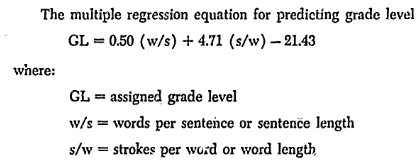
\includegraphics[width=0.7\textwidth]{fig/ari}

    \pause
    \vspace{1em}
    \begin{itemize}
        \item multiplication is implicit in this notation: $ x(\dots) = $ x * (\dots)
        \item mistake in paper! s is both sentences and strokes!
    \end{itemize}
\end{frame}

\begin{frame}[fragile]{From formula to code}
\begin{lstlisting}[language=python]
w = 500
s = 25
c = 3200

result = 0.5 * (w / s) + 4.71 * (c / w) - 21.43
\end{lstlisting}

\pause But why so cryptic?

    Good code has \dots

\begin{itemize}
    \item Clear variable names
    \item Steps that are easy to follow
\end{itemize}
\end{frame}

\begin{frame}[fragile]{Improved version}
\begin{lstlisting}[language=python]
total_words = 500
total_sentences = 25
total_characters = 3200


words_per_sent = total_words / total_sentences
chars_per_word = total_characters / total_words

result = 0.5 * words_per_sent + 4.71 * chars_per_word - 21.43
\end{lstlisting}
\end{frame}


\begin{frame}{How to run Python code}
	\begin{columns}
		\column{0.5\linewidth}
			Traditional method:
			\begin{enumerate}
				\item edit file
				\item run
				\item repeat
			\end{enumerate}
		\column{0.5\linewidth}
			Notebooks
			\begin{itemize}
				\item Notebook: combines text, code, and results
				\item Graphical interface in browser
			\end{itemize}
            [\href{http://mybinder.org/v2/gh/binder-examples/requirements/master}{demo of Jupyter notebook}]
	\end{columns}
\end{frame}



\section{Course overview}
\frame{\tableofcontents[currentsection]}

\begin{frame}{Course overview}
    \begin{itemize}
       \item 7 lectures \& labs
       \item 2 graded assignments \\
           (100\% of final grade)
    \end{itemize}
\end{frame}

\begin{frame}{Learning goals}
    After completing this course you will know the basics of \dots
    \begin{itemize}
        \item Text analysis: cleaning texts, counting words
        \item Exploratory data analysis: load a tabular dataset, create plots
        \item Fixing errors in programs
        \item Reading documentation, collaborating with programmers
    \end{itemize}
\end{frame}


% \begin{frame}{Course materials}
%     \begin{itemize}
%         \item Lectures with our material
%         \item Lab: Notebooks from the course Python for the Humanities
%         \item Preparation for lab:
%             \begin{itemize}
%                 \item Video lectures from the course Hacking the Humanities
%                 \item Textbook: Think Python
%             \end{itemize}
%     \end{itemize}
% \end{frame}

\begin{frame}{Course summary}
    \begin{itemize}
        \item \structure{Programming} is the creative and challenging process
            of writing a program
        \item A program is a sequence of unambiguous executable
            instructions to perform a task
        \item The code of a program is in some programming language
        \item Python is a high-level programming language
    \end{itemize}
\end{frame}

\begin{frame}{Some advice}
    \begin{itemize}
        \item This course gives a lot of (new) information
        \item Information is provided in a \structure{cumulative} way:
            each new piece of information builds on previous information
        \item Watch tutorials, read, and practice
        \item \structure{Ask questions} as soon as you think you are lost!
    \end{itemize}
\end{frame}

\begin{frame}{Code of conduct}
    \begin{itemize}
        \item Read the course manual (syllabus); available on Nestor
        \item On Nestor, under Course Documents, each week has:
            \begin{itemize}
                \item Lecture slides
                \item Lab exercises and assignments
            \end{itemize}
        \item Grades will be on Nestor under My Gradebook
    \end{itemize}
\end{frame}

\begin{frame}{Code of conduct}
    \begin{itemize}
        \item \structure{Don't email} us on course content,
            programming issues, grading, etc.!
        \item For questions and remarks, address us face to face in class
            or make an appointment:
            \begin{itemize}
                \item Van Cranenburgh: office hours, room H1311, 411
                \item Bosveld: office hours, room H1311, 430
                \item Meijerhof; after lab hours, or make appointment
            \end{itemize}
    \end{itemize}
\end{frame}


\begin{frame}{Background reading}
    \begin{itemize}
        \item Downey ch.\ 1 and 2
        \item and/or Zelle sec.\ 2.1--2.5 \\
            (make sure it is the latest edition for Python version 3).
        \item Watch youtube tutorials of "Hacking the Humanities" episode 1--5:
            {\small\url{https://www.youtube.com/playlist?list=PL6kqrM2i6BPIpEF5yHPNkYhjHm-FYWh17}}
    \end{itemize}
\end{frame}

\end{document}
